\chapter{PENGUJIAN DAN ANALISIS}
\label{chap:pengujiananalisis}

% Ubah bagian-bagian berikut dengan isi dari pengujian dan analisis

\section{Visualisasi Hasil Kalibrasi}
\label{sec:visualisasihasil} 

Visualisasi hasil kalibrasi dilakukan dengan cara data pada kamera dengan data pada lapangan. Hal itu dilakukan dengan cara memasukkan data pada kamera ke dalam \emph{Lookup Table} yang telah dibuat sebelumnya. Berikut adalah hasil visualisasi yang didapat. 

\begin{figure}[H]
  \centering
  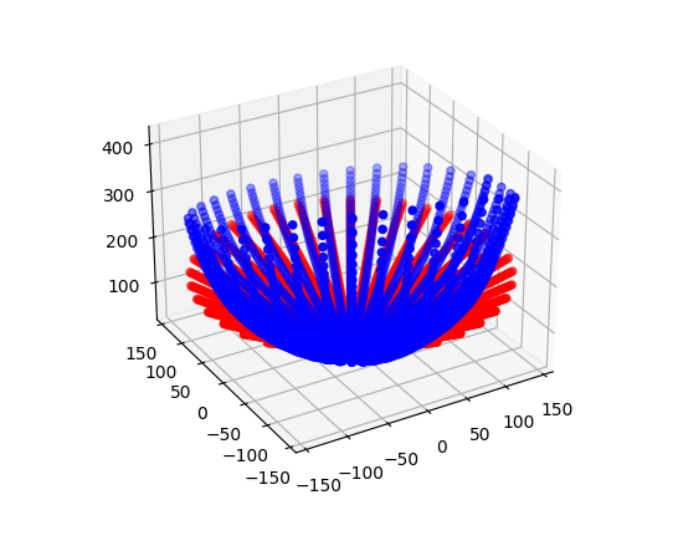
\includegraphics[scale=0.9]{gambar/visual1.png}
  \caption{Visualisasi hasil kalibrasi.}
  \label{fig:hasilkalibrasi}
\end{figure}

Dari gambar tersebut, dapat dilihat bahwa data pada kamera yang digunakan tidak sepenuhnya tegak lurus 90 derajat dengan lapangan. Hal itu terjadi karena kamera yang digunakan tidak terpasang dengan benar. 

\section{Skenario Pengujian Akurasi}
\label{sec:skenariopengujian}

Pengujian dilakukan dengan cara mendeteksi bola yang diam di lapangan dengan memutar robot pada posisinya sendiri. Hal itu membuat robot dapat melihat bola dari berbagai sudut. Pengujian dilakukan dengan mengambil data dari kamera omnivision yang telah terpasang pada robot lalu memroses data tersebut menggunakan \emph{Lookup Table} yang telah dibuat sebelumnya sehingga didapat koordinat bola pada lapangan. Berikut adalah skenario pengujian yang dilakukan: 

\begin{figure}[H]
  \centering
  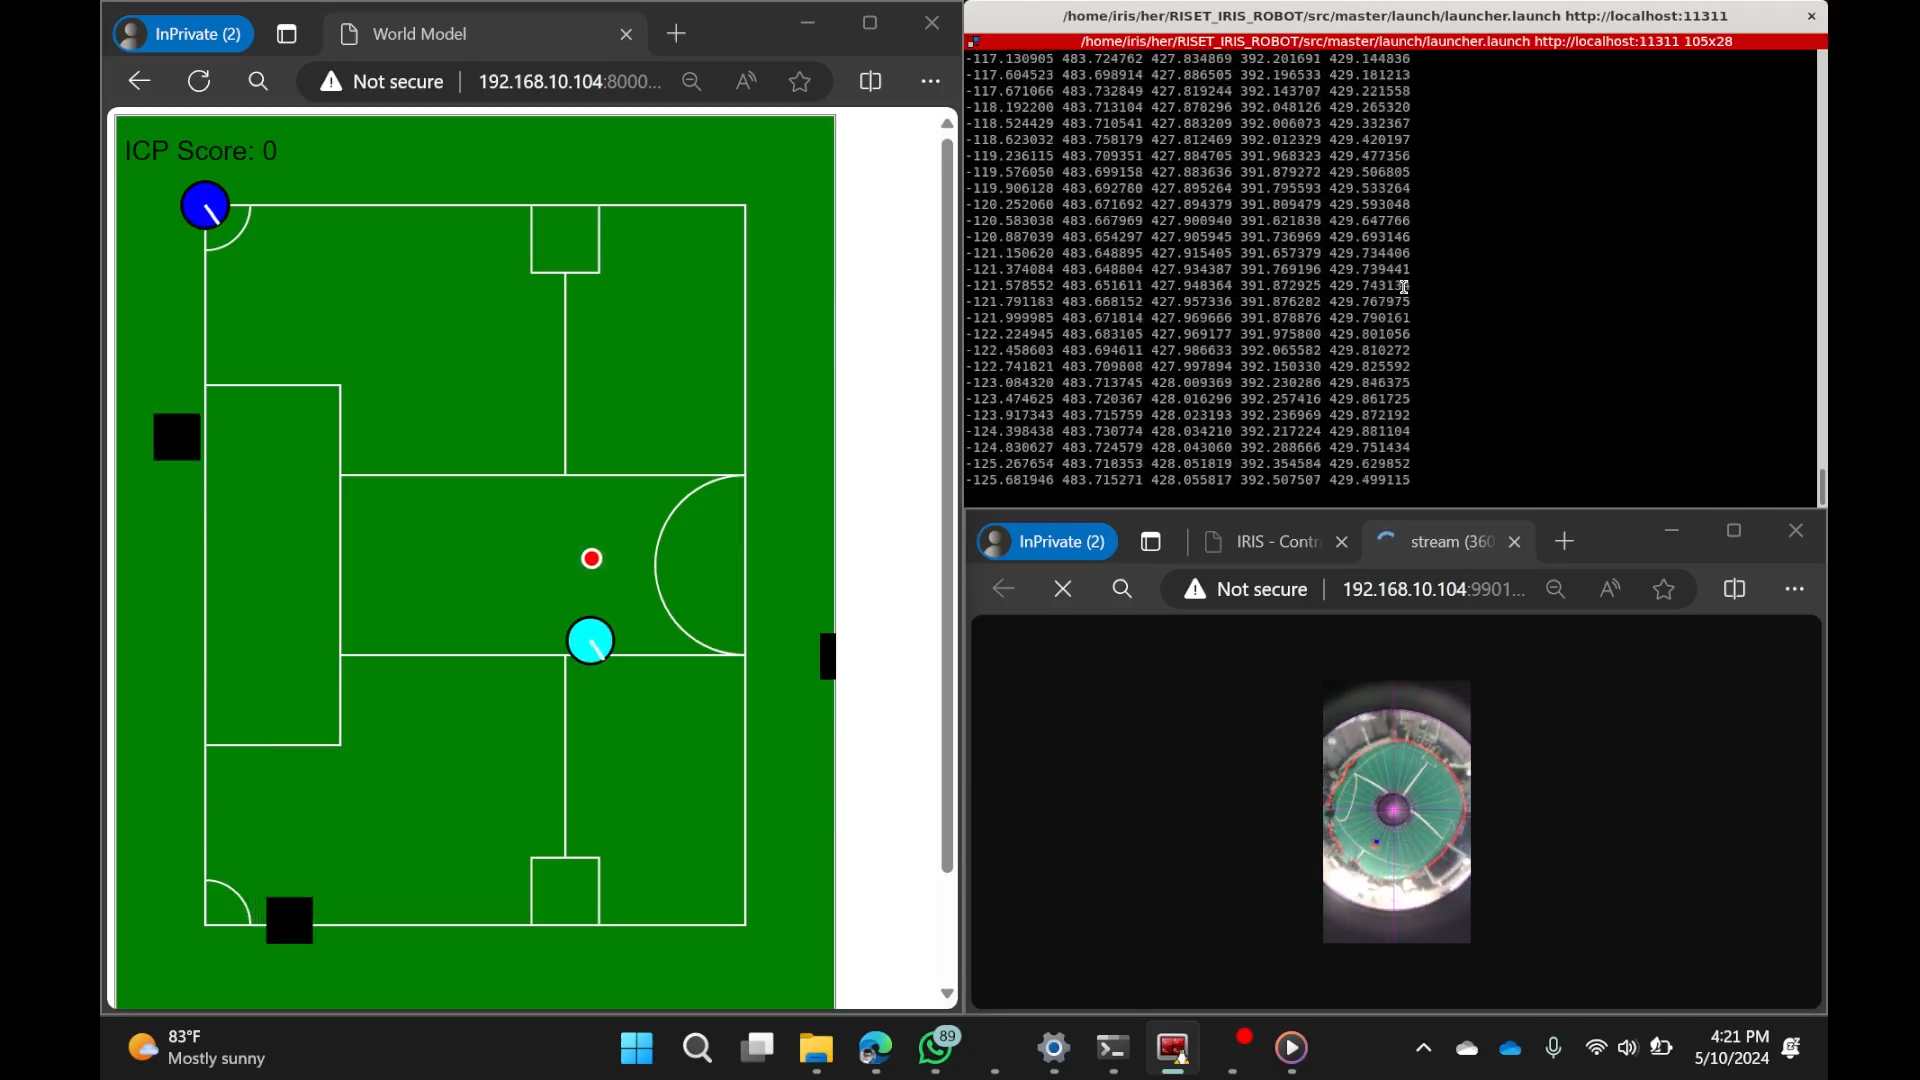
\includegraphics[scale=0.20]{gambar/saat_putar_bola.png}
  \caption{Skenario Pengujian.}
  \label{fig:skenariopengujian}
\end{figure}

Adapun rumusan yang digunakan untuk menghitung posisi bola pada lapangan adalah sebagai berikut: 

\begin{equation}
  \begin{aligned}
    dx &= x\_bola\_cam - x\_center\_cam \\
    dy &= y\_center\_cam - y\_bola\_cam \\
    r\_bola\_cam &= \sqrt{dx^2 + dy^2} \\
    \theta\_bola\_cam &= \arctan(\frac{dy}{dx}) \\
    index &= \theta\_bola\_cam \times r\_max + r\_bola\_cam \\ 
    r\_bola\_lap &= r\_lookup[index] \\
    \theta\_bola\_lap &= \theta\_bola\_cam + robot\_pose\_\theta - 90 \\
    x\_bola &= robot\_pose\_x + r\_bola\_lap \times \cos(\theta\_bola\_lap) \\
    y\_bola &= robot\_pose\_y + r\_bola\_lap \times \sin(\theta\_bola\_lap) \\
  \end{aligned}
\end{equation}

\section{Evaluasi Pengujian Akurasi}
\label{sec:analisispengujian}

Dari pengujian yang telah dilakukan, didapat data sebagai berikut:

% Contoh pembuatan tabel
\begin{longtable}{|c|c|c|}
  \caption{Hasil Pengujian Posisi Bola pada Lapangan}
  \label{tb:posisibolalapangan}                                   \\
  \hline
  \rowcolor[HTML]{C0C0C0}
  \textbf{Sudut Robot ke Bola} & \textbf{Posisi Bola X} & \textbf{Posisi Bola Y} \\
  \hline
  0 deg            & 380.14 cm                & 420.93 cm            \\
  30 deg           & 386.72 cm                & 420.77 cm            \\
  60 deg           & 387.15 cm                & 420.94 cm            \\
  90 deg           & 387.70 cm                & 421.69 cm           \\
  120 deg           & 386.97 cm                & 431.32 cm           \\
  150 deg           & 389.73 cm                & 431.77 cm           \\
  180 deg           & 389.71 cm                & 430.90 cm           \\
  210 deg           & 392.98 cm                & 430.02 cm           \\
  240 deg           & 391.82 cm                & 429.64 cm           \\
  270 deg           & 388.43 cm                & 426.11 cm           \\
  300 deg           & 386.68 cm                & 424.20 cm           \\
  330 deg           & 385.83 cm                & 421.27 cm           \\
  \hline
\end{longtable}

Dari tabel tersebut didapat standar deviasi pada sumbu x sebesar 2.83 cm sedangkan pada sumbu y sebesar 5.71 cm. Hal itu menunjukkan bahwa hasil pengujian yang dilakukan cukup akurat. 

\section{Skenario Pengujian Akurasi Kedua}
\label{sec:skenariopengujian}

Pengujian akurasi kedua adalah dengan cara robot mendeteksi garis dan membuat visualisasi dari garis tersebut. Pengujian dilakukan dengan cara robot diletakkan di daerah lapangan yang dekat dengan garis dan robot akan melihat sekelilingnya.  

\begin{figure}[H]
  \centering
  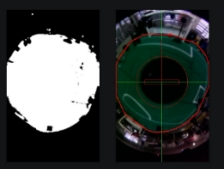
\includegraphics[scale=1.2]{gambar/cam_raw1.jpg}
  \caption{Skenario Pengujian Akurasi Kedua.}
  \label{fig:skenariopengujian}
\end{figure}

Gambar disebelah kiri adalah hasil dari deteksi lapangan yang nantinya akan digunakan untuk mendeteksi garis. Sedangkan gambar disebelah kanan adalah gambar \textit{bgr} dari kamera omnivision. 

\section{Evaluasi Pengujian Akurasi Kedua}
\label{sec:analisispengujian}

Untuk mendapatkan data garis pada lapangan yang telah terdeteksi, maka data tersebut harus dikalkulasi terlebih dahulu. 

\begin{equation}
  \begin{aligned}
    \textbf{Untuk setiap titik pada hasil deteksi garis:} \\
    dx &= x\_titik[i] - x\_center\_cam \\
    dy &= y\_center\_cam - y\_titik[i] \\
    r\_garis\_pcl\_cam &= \sqrt{dx^2 + dy^2} \\
    \theta\_garis\_pcl\_cam &= \arctan(\frac{dy}{dx}) \\
    index &= \theta\_garis\_pcl\_cam \times r\_max + r\_garis\_pcl\_cam \\ 
    r\_garis\_pcl\_lap &= r\_lookup[index] \\
    \theta\_garis\_pcl\_lap &= \theta\_garis\_pcl\_cam + robot\_pose\_\theta - 90 \\
    x\_garis\_pcl[i] &= robot\_pose\_x + r\_garis\_pcl\_lap \times \cos(\theta\_garis\_pcl\_lap) \\
    y\_garis\_pcl[i] &= robot\_pose\_y + r\_garis\_pcl\_lap \times \sin(\theta\_garis\_pcl\_lap) \\
  \end{aligned}
\end{equation}

Dari kalkulasi yang telah dilakukan, didapat data gambar sebagai berikut:

\begin{figure}[H]
  \centering
  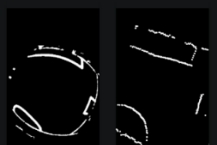
\includegraphics[scale=1.2]{gambar/cam_raw2.jpg}
  \caption{Hasil Pengujian Akurasi Kedua.}
  \label{fig:hasilpengujian}
\end{figure}

Gambar disebelah kiri adalah hasil dari deteksi garis yang dilakukan oleh robot. Hasil garis tersebut merupakan hasil yang sudah diolah dengan hasil deteksi lapangan. Garis tersebut adalah garis yang belum dikalibrasi. Sedangkan gambar disebelah kanan adalah hasil dari garis yang sudah dikalibrasi. 

\section{Skenario Pengujian Kecepatan Komputasi}
\label{sec:analisispengujian}

Pengujian dilkukan dengan cara membandingkan apakah sistem kalibrasi baru lebih cepat dibandingkan menggunakan sistem kalibrasi lama. Pada robot, sistem kalibrasi baru hanya menggunakan sebuah \emph{Lookup Table} yang berisi data kalibrasi kamera, Sedangkan sistem kalibrasi lama menggunakan algoritma \emph{regresi polynomial}. Berikut adalah source code yang digunakan untuk menghitung waktu komputasi dari kedua sistem kalibrasi tersebut: 

\lstinputlisting[
  language=C++,
  caption={Program Uji waktu.},
  label={lst:ujiwaktu}
]{program/test_waktu.cpp}

\section{Evaluasi Pengujian Kecepatan Komputasi}
\label{sec:analisispengujian}

Dari pengujian yang telah dilakukan, didapat data sebagai berikut: 
\begin{figure}[H]
  \centering
  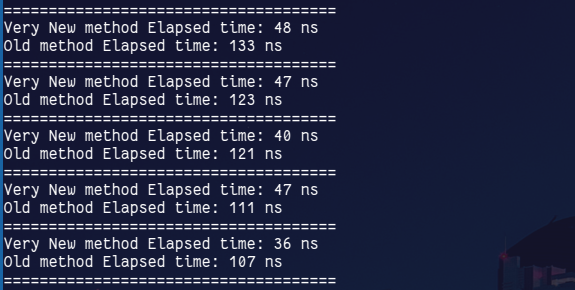
\includegraphics[scale=0.9]{gambar/beda_waktu.png}
  \caption{Evaluasi pengujian waktu.}
  \label{fig:ujiwaktu}
\end{figure}

Dari grafik tersebut dapat dilihat bahwa sistem kalibrasi baru lebih cepat 75.4 ns dibandingkan dengan sistem kalibrasi lama. Dengan rata-rata Kalibrasi baru membutuhkan waktu 43.6 ns sedangkan kalibrasi lama membutuhkan waktu 119 ns. 
